\chapter{Внешний угол треугольника}

\section{Задачи на урок}

\begin{enumerate}

    \item Сформулируйте теорему о соотношении сторон и углов треугольника. Сформулируйте неравенство треугольника 

    \item \textbf{Разминка.} 

    1) Есть палочки с длинами 2, 3, 4, 5, 6 см. Сколько треугольников можно составить из них? (Одну палочку можно использовать для разных треугольников.)

    2) В треугольнике длина одной стороны равна 4, а
другой --- 5. Какие целые значения может принимать длина третьей стороны?


    \item \textbf{Верно ли, что...}

    1) Если внешний угол при вершине $A$ треугольника $ABC$ равен $120^\circ$, а внутренний угол B равен $50^\circ$, то сторона $AB$ является самой короткой в этом треугольнике.

    2) В $\triangle{ABC}$, если $\angle{A}>\angle{B}$, то высота из $A$ больше высоты из $B$.

    3) Если периметр равнобедренного треугольника равен 25, а одна сторона равна 5, то другая сторона обязательно равна 10.

    \item \textbf{Задачи на соотношение элементов треугольника.} 
    
    1) В равнобедренном треугольнике $ABC$ $(AB=AC)$ внешний угол при вершине $C$ равен $110^\circ$. На продолжении стороны $CB$ за точку $B$ отметили точку $D$, а на продолжении стороны $BC$ за точку $C$ --- точку $E$ так, что $BD=CE$. Известно, что $\angle{DAE}=130^\circ$. Найдите $\angle{CAE}$.

    2) Докажите, что если в $\triangle{ABC} \; AB>AC$, $AD$ --- биссектриса ($D\in{BC}$), то $BD>DC$.

    \textit{Подсказка.} Дополнительное построение: на стороне $AB$ от точки $A$ отложите отрезок, равный $AC$.

    \item \textbf{Внешний угол треугольника.} Теория:

    1) Внешний угол треугольника равен сумме двух внутренних углов, не смежных с ним. 

    2) Биссектрисы внутреннего и внешнего угла треугольника перпеникулярны.

    3) Биссектриса внешнего угла треугольника параллельна противоположной стороне треугольника тогда и только тогда, когда треугольник равнобедренный.

    \item \textbf{Задача на внешний угол треугольника.} В р/б $\triangle{ABC}$ с основанием $AC$ на стороне $AB$ отмечена точка $D$, на стороне $BC$ отмечена точка $E$ так, что $BD=DE=EA=AC$. Найдите градусную меру $\angle{B}$.
\end{enumerate}

\newpage

\section{Комментарии}

\begin{enumerate}

\item Теорема о соотношении углов и сторон треугольника. В любом треугольнике: 1) против большей стороны лежит больший угол; 2) против большего угла лежит большая сторона.

Неравенство треугольника. В треугольнике сумма длин любых двух сторон больше длины третьей стороны.

\item 1) 7 треугольников; \quad 2) от 2 до 8. 

\item 1) Неверно, сторона $AB$ самая длинная. 

2) Неверно, например, если $\angle A$ тупой. (На самом деле, это утверждение неверно всегда: к большей стороне проведена меньшая высота).

3) Верно. Если 5 --- основание, то боковые стороны равны 10. Такой треугольник существует (проверяем по неравенству треугольника). Если 5 --- боковая сторона, то основание 15, и треугольник 5-15-15 не существует.

\item Дано: $AB=AC$, $BD=CE$, $\angle{ACE}=110^\circ$, $\angle{DAE}=130^\circ$. Найти: $\angle{CAE}$.

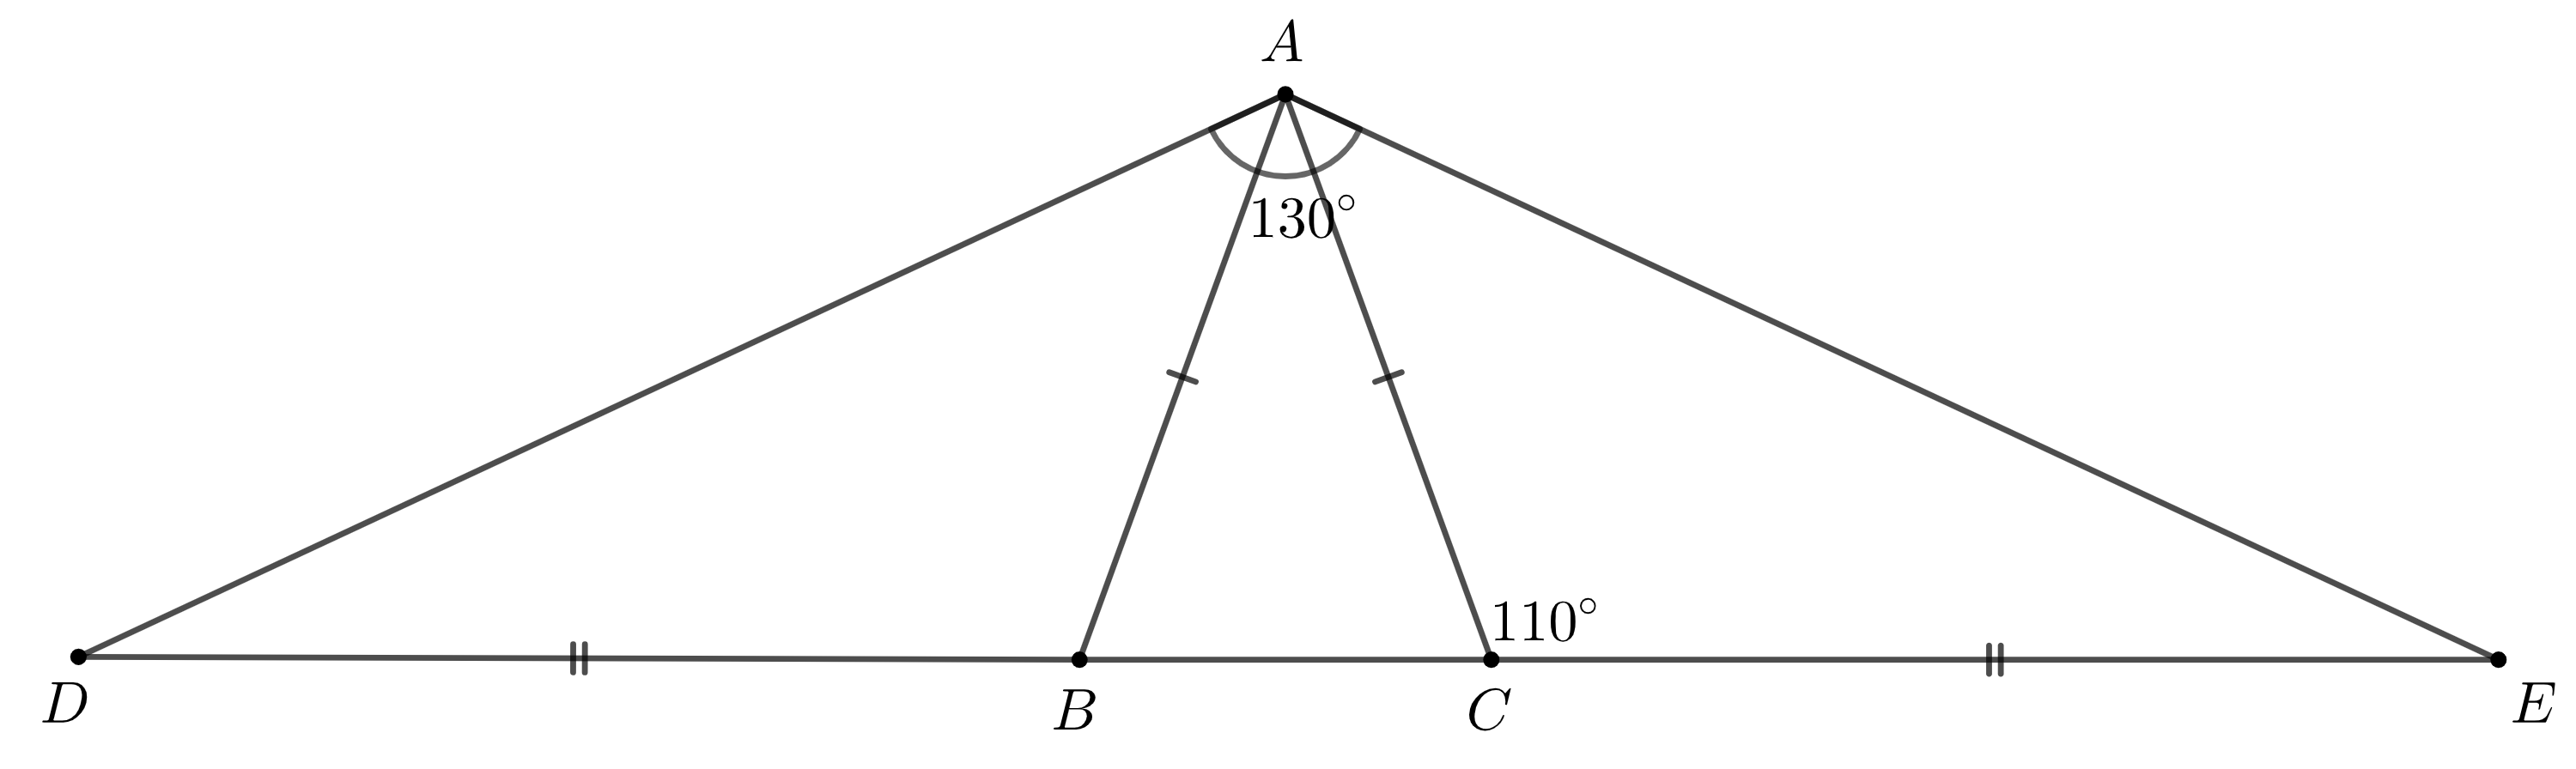
\includegraphics[width=.9\textwidth]{2026_geom/pic/2_01.png}

1) $\angle ACB=70^\circ$ (со свойству суммы смежных углов). $\angle ABC=\angle{ACB}=70^\circ$ (по свойству р/б $\triangle ABC$).

3) $\angle{BAC}=40^\circ$ (по свойству суммы углов треугольника).

4) $\triangle{ABD}=\triangle{ACE}$ (по I признаку: $BD=CE$, $AB=AC$ по условию, $\angle ABD=\angle ACE$ как смежные с равными). Тогда $AD=AE$ как соответственные стороны.

5) По свойству р/б $\triangle{ADE}$ $\angle{A}=\angle{E}=\dfrac{180^\circ-130^\circ}{2}=25^\circ$.

6) В $\triangle{AEC}$ $\angle CAE=180^\circ-110^\circ-25^\circ=45^\circ$.

\noindent \textit{Ответ:} $\angle{CAE}=45^\circ$.

\item Дано: $\triangle ABC$, $AB>AC$, $AD$ --- биссектриса. Доказать: $BD>DC$.

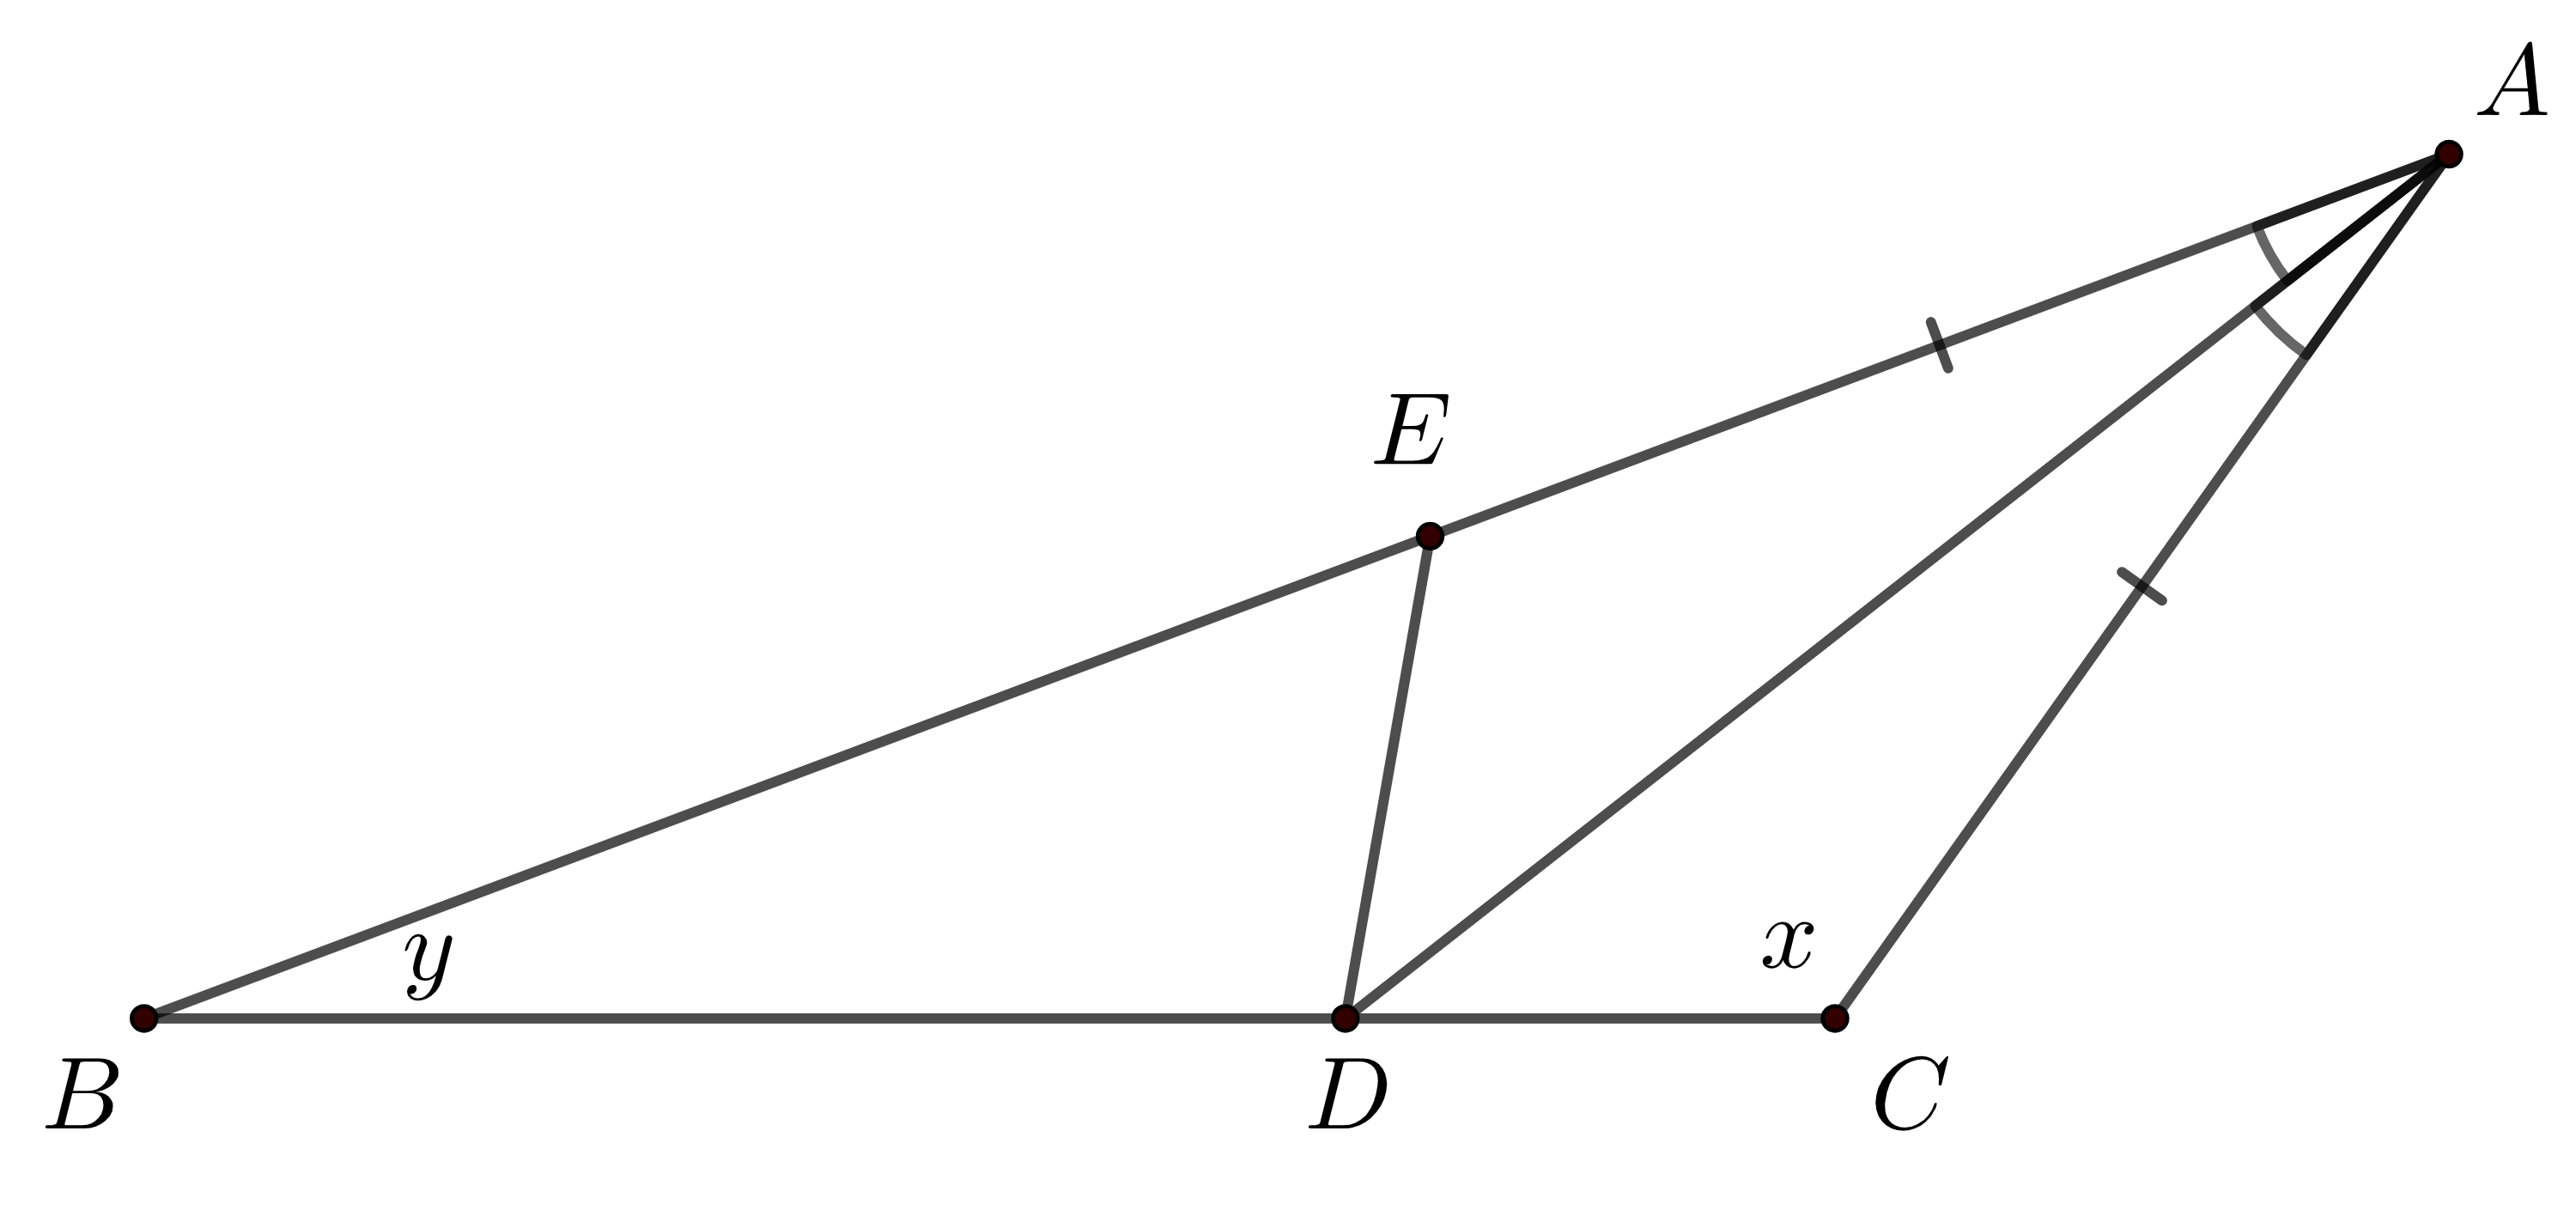
\includegraphics[width=.6\textwidth]{2026_geom/pic/2_02.png}

1) Отложим на стороне $AB$ отрезок $AE$, равный $AC$.

2) $\triangle{ADE}=\triangle{ADC}$ по I признаку. Пусть $\angle{ACD}=\angle{AED}=x$, $\angle B=y$.

3) Нужно доказать, что в $\triangle{BED}$ $BD>DE$ (так как $DE=DC$). То есть нужно доказать, что $\angle{BED}>\angle{B}$, то есть $180^\circ -x>y$. 

4) Это неравенство легко получить из неравенства $x+y<180^\circ$ (это верно, т.к. $x$ и $y$ - два угла треугольника). Значит, $\angle BED > \angle B \Longrightarrow BD > ED \Longrightarrow BD > DC$, что и требовалось доказать.

\end{enumerate}

\begin{enumerate}

    \setcounter{enumi}{5}

\item Дано: $AB=BC$; $BD=DE=AE=AC$. Найти: $\angle{B}$.

\noindent\begin{minipage}{.7\textwidth}
1) Обозначим $\angle{B}=x$. Тогда в р/б $\triangle{BDE} \; \angle DEB=x$.

\smallskip

2) $\angle ADE=2x$ (внешний угол $\triangle{ADE}$). $\angle{EAD}=2x$ (по св-ву р/б $\triangle DAE$).

\smallskip

3) В $\triangle DAE \; \angle{DEA}=180^\circ-4x$.

\smallskip

4) $\angle{CEA}=180^\circ-(180^\circ-4x)-x=3x$ (сумма трёх углов с вершиной $E$ равна $180^\circ$).

\smallskip

5) В р/б $\triangle AEC \; \angle C = \angle{AEC}=3x$.

\smallskip

6) $\triangle{ABC}: \; x+3x+3x=180^\circ \Longrightarrow x=\dfrac{180^\circ}{7}$.

\smallskip

\textit{Ответ:} $\dfrac{180^\circ}{7}$.
\end{minipage}%
\begin{minipage}{.3\textwidth}
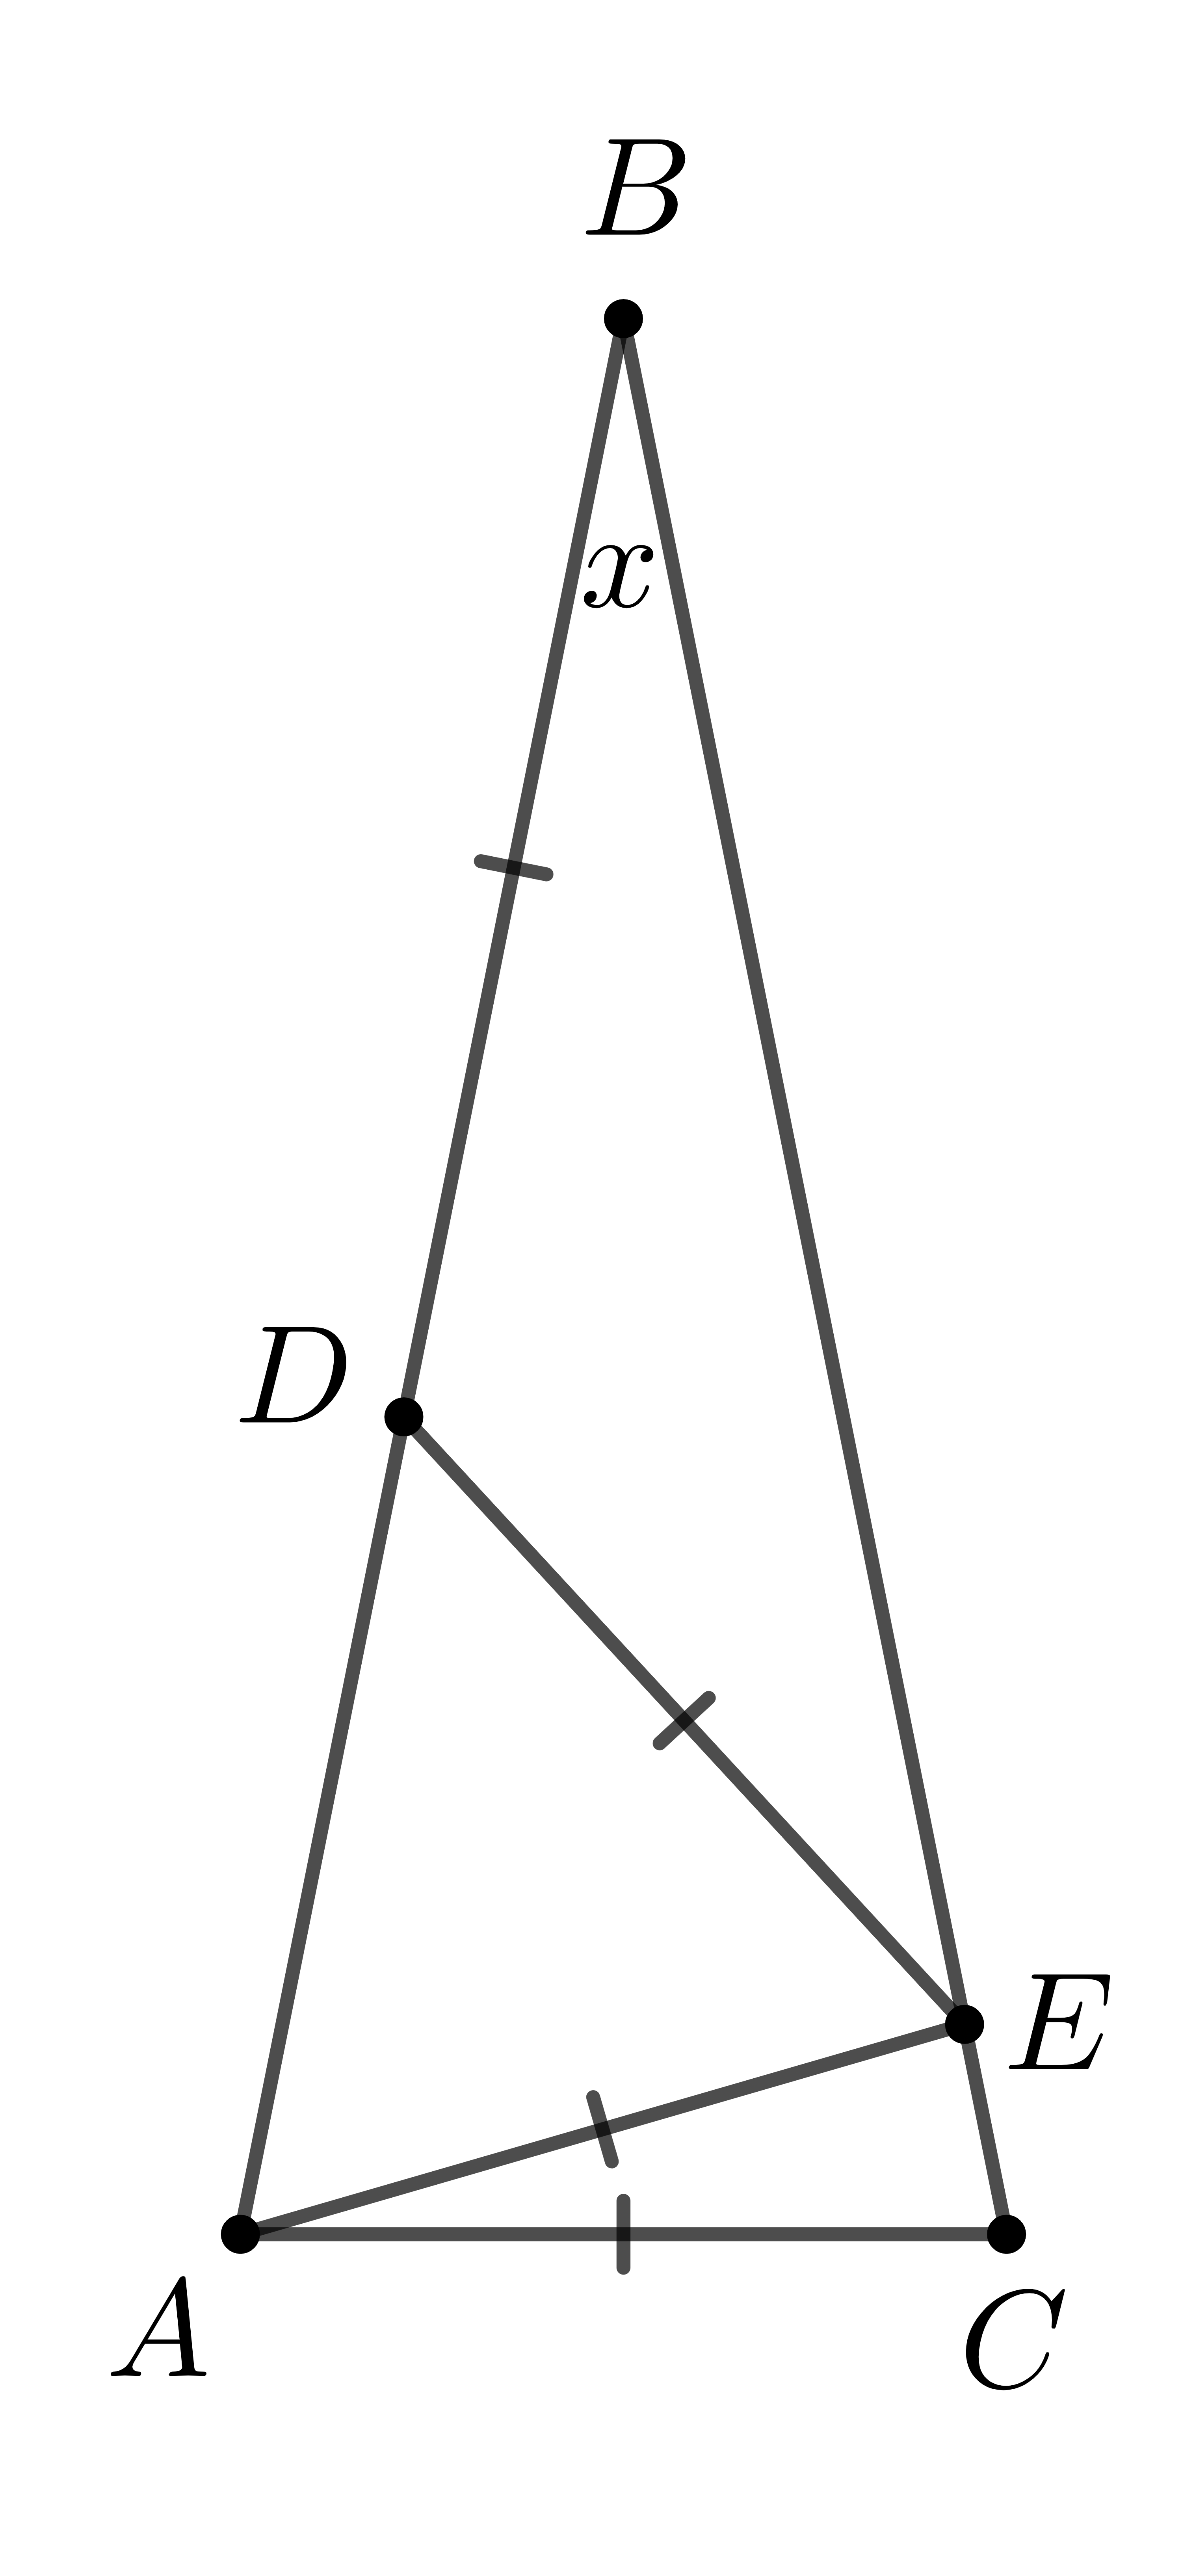
\includegraphics[width=.8\textwidth]{2026_geom/pic/2_03.png}
\end{minipage}



\end{enumerate}

\newpage

\section{Домашнее задание}

\begin{enumerate}
    \item Все утверждения ниже \textbf{неверны.} Приведите опровергающий рисунок к каждому из них.

    1) Если две стороны и угол одного треугольника равны двум сторонам и углу другого треугольника, то такие треугольники равны.

    2) Если треугольники $ABC$ и $ADC$ прямоугольные и равнобедренные, то $AC=AD$.

    3) Если одна сторона треугольника в два раза больше другой, то и противолежащий ей угол в два раза больше угла, лежащего против второй стороны.

    \item \textbf{Задачи только с ответом или рисунком.} 
    
    1) Нарисуйте тупоугольный треугольник и проведите все три его высоты. 

    2) Найдите сумму внешних углов треугольника (для каждого внутреннего угла берётся один внешний). 

    3) В треугольнике два угла равны $20^\circ$ и $60^\circ$. Разрежьте его на два равнобедренных треугольника.

    \item Докажите \textbf{свойство биссектрисы внешнего угла равнобедренного треугольника:}

    Биссектриса внешнего угла, прилежащего к основанию равнобедренного треугольника,  параллельна его боковой стороне.

    \item Докажите \textbf{признак равнобедренного треугольника:}

    Если биссектриса внешнего угла треугольника параллельна стороне, противолежащей соответственному внутреннему углу, то треугольник равнобедренный.

    \item В $\triangle{ACD}$ с прямым углом $C$ проведена высота $CD$. $CE$ --- биссектриса треугольника $ACD$. Докажите, что $BC=BE$.

    \item В треугольнике $ABC$ угол $A$ равен $\alpha$. Биссектриса угла $B$ и биссектриса внешнего угла $C$ пересекаются в точке $D$. Найдите угол $BDC$. (Выразите его через $\alpha$.)

\end{enumerate}